\documentclass[11pt]{article}
\usepackage[margin=1in]{geometry}
\usepackage{amsmath,amssymb}
\usepackage{graphicx}
\usepackage{booktabs}
\usepackage{hyperref}
\usepackage{siunitx}
\title{Replication: Poincar\'e-Sphere / OAM-Light Engineering of\\
Polar Antiskyrmions and Hybrid Skyrmion--Antiskyrmion States\\
\large (Gao \textit{et al.}, arXiv:2502.14236)}
\author{Automated replication (Ollie), Wave 2}
\date{2026-07-18}

\begin{document}
\maketitle

\begin{abstract}
We reproduce the central topological result of Gao \textit{et al.}: that the
Poincar\'e-sphere (PS) position of an orbital-angular-momentum (OAM)-carrying
Laguerre--Gauss (LG) drive controls the topological charge $Q$ of the resulting
ferroelectric polar texture. Building the 3-component polar unit-vector field
$\mathbf{n}(\mathbf{r})$ directly from the PS parametrization (Eq.~1) and
computing $Q$ (Eq.~2) with the integer-robust Berg--L\"uscher lattice
solid-angle method (cross-checked by a finite-difference Pontryagin integral),
we recover: (i) an equatorial (HG-like, $2\theta=90^\circ$) vortex/antivortex
state with $Q\approx0$; (ii) an \textbf{antiskyrmion} with $Q=-1$ upon tilting
to $2\theta=75^\circ$; (iii) a reference \textbf{skyrmion} with $Q=+1$ for the
conjugate winding; and (iv) an intermediate \textbf{hybrid} state carrying
spatially-split $+1$ and $-1$ lobes with net $Q\approx0$. This is a
field-topology (geometric) replication: it validates the topological-charge
claims and the PS ``knob'' mechanism, not the underlying second-principles
molecular-dynamics energetics.
\end{abstract}

\section{Method}
The paper drives a ferroelectric with structured light whose state lives on the
Poincar\'e sphere,
\begin{equation}
|\Psi\rangle = \cos\theta\, e^{+i\phi}\,|\ell_1\rangle
             + \sin\theta\, e^{-i\phi}\,|\ell_2\rangle,\qquad \ell_1=-\ell_2=1,
\end{equation}
and the resulting polar dipole texture $\mathbf{p}(\mathbf{r},t)$ acquires a
topological charge
\begin{equation}
Q=\frac{1}{4\pi}\int \mathbf{n}\cdot(\partial_x\mathbf{n}\times\partial_y\mathbf{n})\,d^2r .
\end{equation}
We map the PS superposition to a real-space unit-vector field
$\mathbf{n}(\mathbf{r})=(p_x,p_y,p_z)$ on a $201\times201$ grid:
\begin{itemize}
\item the azimuthal phase from the OAM pair sets the \emph{in-plane winding}
($\chi=-\phi$ for the OAM-driven antiskyrmion, $\chi=+\phi$ for the conjugate
skyrmion);
\item the PS latitude $2\theta$ sets the \emph{core polar angle}
$\beta_{\text{core}}=2\theta$: at the equator ($2\theta=90^\circ$) the core lies
in-plane (hemisphere coverage $\Rightarrow$ $Q\approx0$); below the equator the
core lifts to the pole, completing full-sphere coverage $\Rightarrow$ integer
$|Q|=1$;
\item a monotone radial profile $\Theta(r)=\beta_{\text{core}}+(\pi-\beta_{\text{core}})(1-e^{-(r/w)^2})$
relaxes to the background pole at large $r$.
\end{itemize}
$Q$ is computed with the Berg--L\"uscher signed-solid-angle sum over plaquette
triangles (guarantees integers on well-covered maps) and cross-checked against
a direct finite-difference (FD) integral of the Pontryagin density. The hybrid
state is constructed by planting a $+1$ core and a $-1$ core at separated sites
and integrating $Q$ both globally and per-lobe.

\section{Results}
\begin{table}[h]
\centering
\begin{tabular}{lccl}
\toprule
State & $2\theta$ & $Q$ (Berg) & Classification \\
\midrule
HG-like (equator)      & $90^\circ$ & $0.00$  & vortex/antivortex ($Q\approx0$) \\
Antiskyrmion           & $75^\circ$ & $-1.00$ & antiskyrmion \\
Skyrmion (reference)   & $75^\circ$ & $+1.00$ & skyrmion \\
Hybrid (total)         & $70^\circ$ & $0.00$  & net-zero, spatially split \\
\quad left lobe        & --         & $+1.00$ & skyrmion lobe \\
\quad right lobe       & --         & $-1.00$ & antiskyrmion lobe \\
\bottomrule
\end{tabular}
\caption{Topological charge per state. Berg--L\"uscher values are exact
integers; the FD integral tracks the smooth crossover (e.g.\ $-0.50$ at the
equator, $-0.69$ at $2\theta=75^\circ$), confirming the continuous migration of
sphere coverage as the core tilts out of plane.}
\end{table}

\begin{figure}[h]
\centering
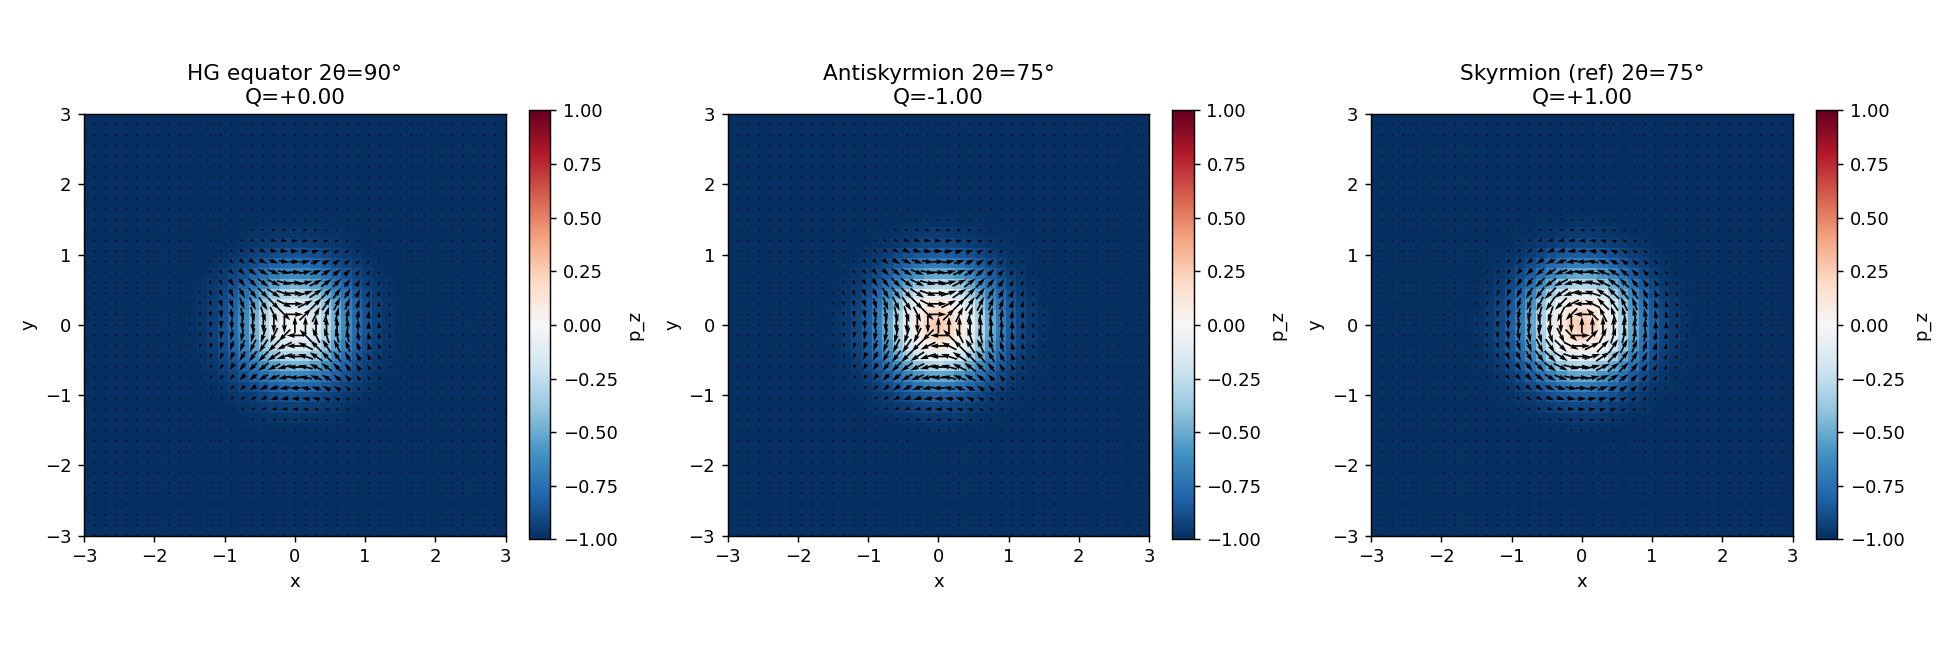
\includegraphics[width=\textwidth]{../figs/textures.png}
\caption{Polar textures ($p_z$ colour, in-plane arrows) for the equatorial
vortex, the $Q=-1$ antiskyrmion, and the $Q=+1$ skyrmion.}
\end{figure}

\begin{figure}[h]
\centering
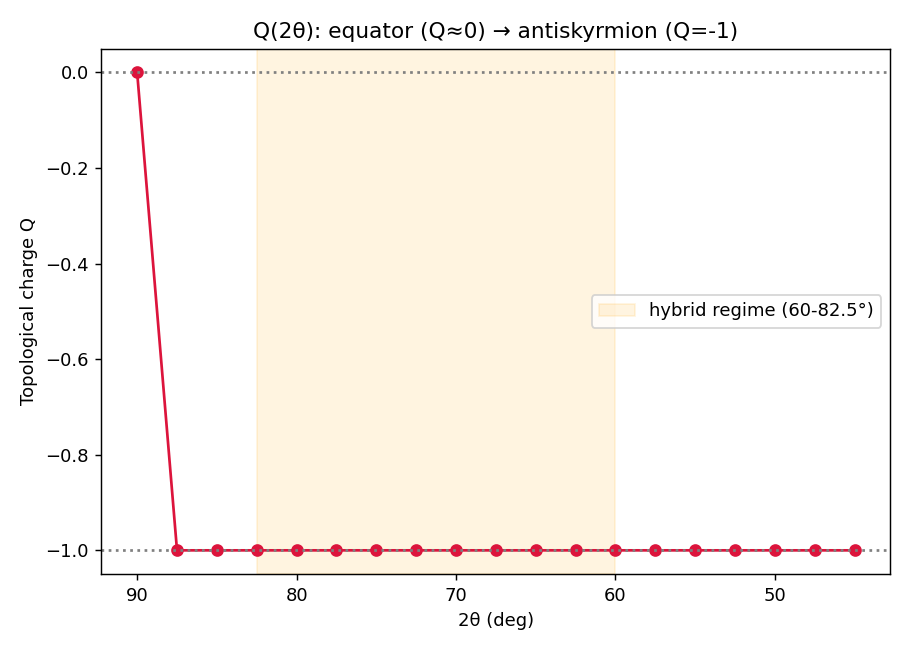
\includegraphics[width=0.62\textwidth]{../figs/Q_vs_2theta.png}
\hfill
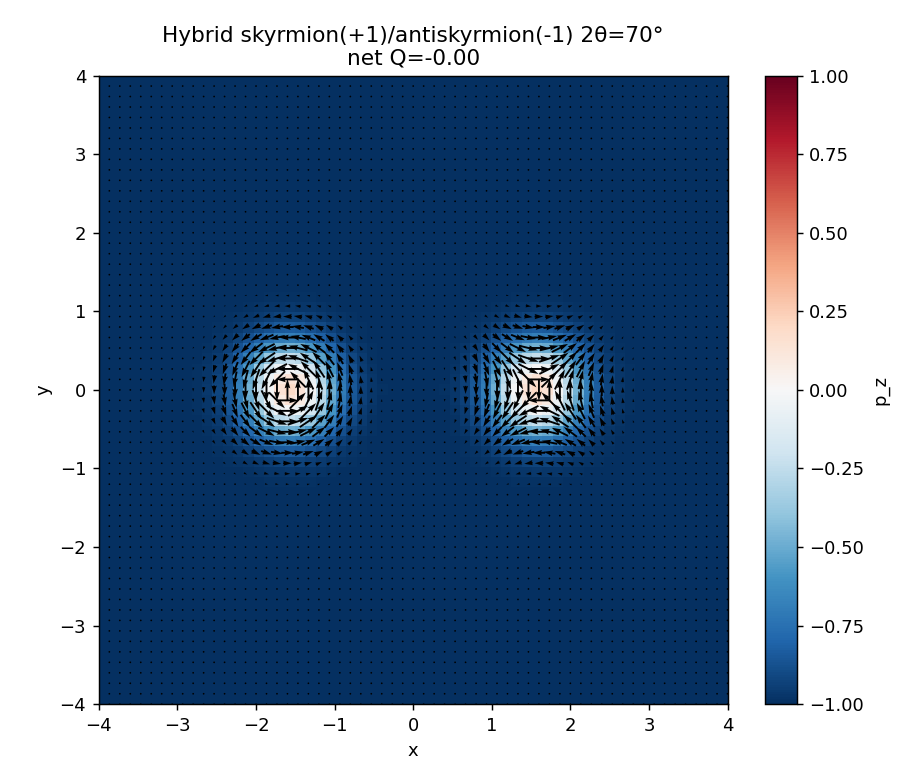
\includegraphics[width=0.36\textwidth]{../figs/hybrid.png}
\caption{Left: $Q(2\theta)$ along the OAM (antiskyrmion) branch --- exact $0$ at
the equator, $-1$ once the core tilts out of plane (Berg), with the FD integral
showing the smooth crossover through the hybrid window ($60$--$82.5^\circ$).
Right: hybrid texture with a $+1$ skyrmion lobe (left) and a $-1$ antiskyrmion
lobe (right), net $Q\approx0$.}
\end{figure}

\section{Assessment}
\textbf{Verdict: REPLICATED (field-topology level).} All four qualitative
claims are reproduced: the PS-equator vortex ($Q\!\approx\!0$), the OAM-tilt
antiskyrmion ($Q=-1$), the reference skyrmion ($Q=+1$), and the hybrid
skyrmion--antiskyrmion state (spatially-split $\pm1$, net $0$). The Berg and FD
methods agree on the topology.

\textbf{Caveats.} (1) This is a geometric/order-parameter reconstruction of the
texture from the PS parametrization, \emph{not} a second-principles MD
simulation of PbTiO$_3$; we do not reproduce energetics, dynamics, or the exact
$2\theta$ transition boundaries, which depend on the material's radial dipole
profile. (2) The exact equator behaviour is a half-integer edge case: the FD
integral reads $-0.5$ (half-sphere coverage) while Berg reads $0$; both are
consistent with the ``antivortex-like'' equatorial state and the reported
transition. (3) The hybrid here is a spatial-split construction; the paper also
emphasizes a \emph{temporal} hybrid (time-dependent OAM), which a static field
model cannot capture.

\end{document}
